%!TEX root = ../final_report.tex


\subsection{Framework}
This project is implemented based on Keras framework \cite{Chollet2015_keras}, which is a modular neural network library. The library is written in Python and can run on top of Theano or TensorFlow. In this project, we propose to use Theano backend \cite{theano2016} for implementation.

Since we need to use pretrained weights from AlexNet, our system has to be able to load this network. However, AlexNet is provided under caffemodel format, which is used in CaffeNet-based deep learning networks \cite{Jia2014_caffe}. The problem is original Keras framework does not allow to load caffemodel directly. Therefore, we use a modified version of Keras, provided by Sol\`{a} \cite{Sola2016}. This version includes a fully functional Keras framework with an additional package for converting from caffemodel to keras format.



\subsection{Implementation}
The project contains 4 main modules: data processor, model architecture, model training, and model testing.

\subsubsection{Data Processor}
The module takes care of loading and preprocessing input data. The input data are cropped with respect to the ground truth segmentation mask beforehand, as showed in Figure \ref{fig:img_cropped}. For preprocessing task, inputs undergo the procedure introduced in Section \ref{subsec:preprocessing}: images are resized efficiently to the size of 227x227 (based on Equation \ref{equ:rescale}) and depth maps have an additional step of colorizing. 

For data loading, the module receive a batch of image, a dictionary list (containing all possible categories), and location of data. Since the amount of data is significant, we cannot load everything at the same time, therefore batch processing is necessary. Based one the naming format of each sample in the batch (Section \ref{subsec:dataset}), we can easily figure out which category that sample belong to and construct the label vector according to the given dictionary
as seen in Equation \ref{equ:label}. Since we are using pretrained weights from AlexNet to train the network, it is essential to remove the mean image \footnote{A mean image for AlexNet under NumPy format is available at: \url{https://github.com/BVLC/caffe/blob/master/python/caffe/imagenet/ilsvrc_2012_mean.npy}.} of ImageNet from every input after loading.

\subsubsection{Model Architecture}
This module creates the architecture for the stream and fusion networks. Common Keras-based systems are implemented based on Sequential model, which allows adding layers in a sequential manner. Such scheme of architecture is actually found in popular network, such as AlexNet \cite{Krizhevsky2012_alexnet}, VGG \cite{Simonyan2014_vgg}. However, such architecture faces the problem of constructing fusion layer. Although Keras provides layer called Merge layer to concatenate different sources of input, it does not work well with Sequential model, making it impossible to load networks after training. To overcome this problem, we use Graph models instead, which offers more flexibility but still retains core functionalities as in Sequential models.

The module has two main parts: the first one replicates the network architecture of AlexNet and the second one constructs the fusion network from stream models. The detail of stream model is illustrated in Figure \ref{fig:single_stream_layout}. Note that we use the same network architecture for both color and depth inputs. Since Keras' Graph models are heavily based on naming convention (each layer is represented as a node and the relationship between different nodes is defined using their names), we include a tag name, being \texttt{\_rgb} or \texttt{\_dep}. Using those tags, we can distinguish the color from depth streams while fusing. For the second part, the module receives color and depth stream (already trained) as inputs and duplicates from layer \textit{fc1} to \textit{fc7} and add parameter \texttt{trainable = False} for convolutional and normalization layers. This helps freezing the trained weights of those layers, making the fusion network focus on training fusion layer only.

After merging outputs from stream models and dense sampling with 4096 nodes, we add another Dense sampling layer that produces 51 nodes, corresponding to 51 categories (as seen in Figure \ref{fig:network}), for classification. This classification layer requires \texttt{softmax} function as activation. In Keras, there are two ways to declare activation for a layer. The first way is to define activation while adding the node
\begin{verbatim}
model.add_node(Dense(nb_classes, activation='softmax'), \
               name='softmax_fus', input='fc1_fus')
model.add_output(name='output', input='softmax_fus')
\end{verbatim}
The second way is to refactor the activation function as a separate node
\begin{verbatim}
model.add_node(Dense(nb_classes), name='fc2_fus', input='fc1_fus')
model.add_node(Activation('softmax'), name='softmax_fus', \
               input='fc2_fus')
model.add_output(name='output', input='softmax_fus')
\end{verbatim}
Although they look similar, the difference actually affect the results significantly. A more detailed explanation on its effect is presented in Section \ref{subsec:exp_result}.

\subsubsection{Model Training}
This module trains all models, including color stream, depth stream, and fusion network. Stream models are trained first then the fusion one. After finishing training, a model is saved for future use as two different files: a \texttt{.json} file to store a json query indicating model's structure and a \texttt{.h5} to store model's weights under HDF5 format. This process is done easily by Keras' provided functions: \texttt{to\_json()} and \texttt{save\_weights()}.

Training process is conducted as several epochs. For each epoch, the training samples are shuffled once to guarantee network's generosity. After training, the model is evaluated on evaluation samples to compute its loss and prediction accuracy. The system is equipped with an early stopping mechanism: if there is no improvement in accuracy (or if the improvement is too insignificant) for $K$ continuous epochs, the training process is halted. The value $K$ is called training's \texttt{patience} and is set as 10.

\subsubsection{Model Testing}
The testing process is similar to evaluation. In this module, the trained model is tested on testing samples, which are separated from training and evaluation set. Models are loaded using Keras' functions \texttt{model\_from\_json()} and \texttt{load\_weights()}. To fully analyze system's performance, the module tests prediction accuracy on all three models: color, depth, and fusion. Detailed results are provided in Section \ref{subsec:exp_result}.

\subsection{Experimental Results}
\label{subsec:exp_result}

To conduct the experiment, we divide RGB-D object data set into three different parts, corresponding to training, evaluation, and testing. As showed in Section \ref{subsec:dataset}, each category contains different objects with some specific ID. For every category, we randomly choose an object for evaluation and another one for testing, while the rest is used for training. Since the number of objects varies for every category, the amount of training object also differs. The generated samples for training, evaluation, and testing are saved as lists for later reuse.

Figure \ref{fig:intermediate_result} displays intermediate outputs at the first and fifth activation layers (using ReLu function), given an apple as input. Figure \ref{fig:intermediate_result}a and \ref{fig:intermediate_result}c are the visualizations of color image while Figure \ref{fig:intermediate_result}b and \ref{fig:intermediate_result}c are those of depth. It is clear that the object's shape is retained on both channels and the features get more complicated at deeper layers. Despite adding artificial information (depth colorizing), things we would expect to see like edge and magnitude detection are still present in the activations.

\begin{figure}
	\centering
	\begin{subfigure}[b]{0.45\linewidth}
		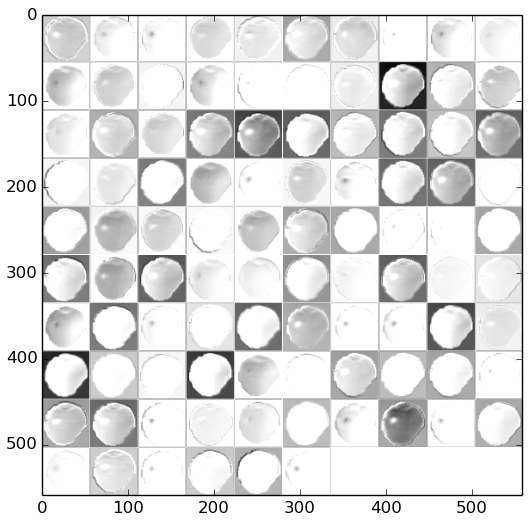
\includegraphics[width=\textwidth]{img/relu1_rgb.png}
		\caption{Activation of ReLU1 layer for RGB image}
	\end{subfigure}   	
	\begin{subfigure}[b]{0.45\linewidth}
		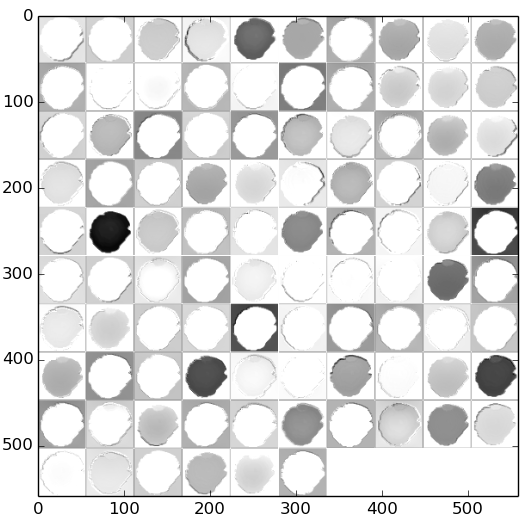
\includegraphics[width=\textwidth]{img/relu1_dep.png}
		\caption{Activation of ReLU1 layer for Depth image}
	\end{subfigure}
	
	\begin{subfigure}[b]{0.45\linewidth}
		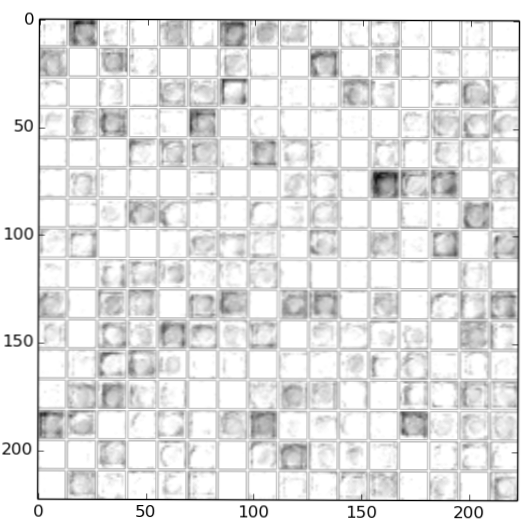
\includegraphics[width=\textwidth]{img/relu5_rgb.png}
		\caption{Activation of ReLU5 layer for RGB image}
	\end{subfigure}   	
	\begin{subfigure}[b]{0.45\linewidth}
		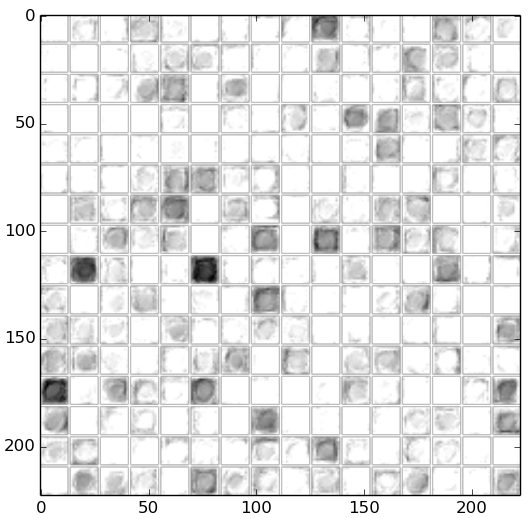
\includegraphics[width=\textwidth]{img/relu5_dep.png}
		\caption{Activation of ReLU5 layer for Depth image}
	\end{subfigure}
	\caption{Visualization of intermediate results on the first and fifth ReLU layers on both RGB and depth images of an apple.}
	\label{fig:intermediate_result}
\end{figure}

Prediction accuracy of the system is presented in Table \ref{tab:result}. We conduct experiences in three different scenarios: reduced data (with 5 classes), full dataset (with 51 classes), and full dataset with refactored fusion layers. Accuracy on stream models are satisfactory and stable, around 68\% for RGB stream and 79\% for depth stream. Fusion network, however, has poorer accuracy. Although it is 56.52\% on reduced dataset, the accuracy drops to 8.07\% on the full one. 

\begin{table}
	\centering
	\caption{Recognition accuracy on reduced (5 categories) and full dataset (51 categories) for RGB stream, depth stream, and fusion network}
	\label{tab:result}
	\begin{tabular}{|c|c|c|c|}
		\hline
		& RGB stream & Depth stream & RGB-D fusion network \\ \hline
		Reduced dataset & 68.26\% & 74.43\% & 56.52\% \\ 
		Full dataset & 68.93\% & 79.19\% & 8.07\% \\ 
		Full dataset with refactored fusion layers & 68.93\% & 79.19\% & 17.34\% \\ \hline
	\end{tabular}
\end{table}

The effect is illustrated with better insight in Figure \ref{fig:prediction}, where prediction is computed on 200 samples randomly selected from testing set. As the figure shows, most of the samples are classified into two classes although the groundtruth labels are well distributed among different categories. However, if we use refactored script for fusion layers, the prediction is better distributed, as showed in Figure \ref{fig:prediction_refactored}. Therefore, we suspect that the problem is caused by some API bug in Keras framework.

\begin{figure}
	\centering
	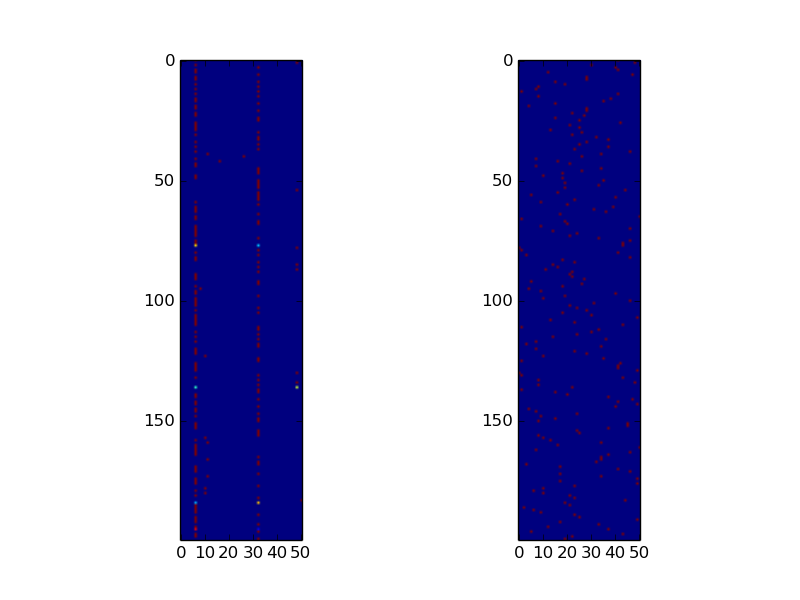
\includegraphics[width=\textwidth]{img/prediction.png}
	\caption{Prediction results (left) and ground truth labels (right) on 200 random samples with unfactored fusion layer.}
	\label{fig:prediction}
\end{figure}

\begin{figure}
	\centering
	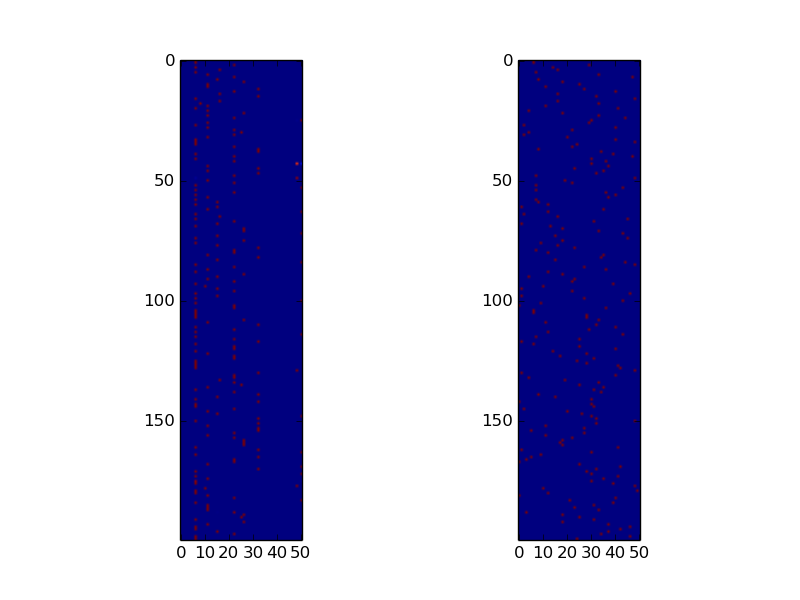
\includegraphics[width=\textwidth]{img/prediction_refactored.png}
	\caption{Prediction results (left) and ground truth labels (right) on 200 random samples with refactored fusion layer.}
	\label{fig:prediction_refactored}
\end{figure}